\usecasedesc{News management}
{
  The news will show the user what is new (change in the application, new recipes, new partner). It can be modified (created, updated) by administrators only. They will be able to specify a title, a description, and a picture if they want. They also will be able to display or not the news to the users.

  \image{newsManagement}{0.75}{News management}{newsManagement}
}
{
  This use case starts when the administrator wishes to add, change, and/or display a news from the system.

  The system requests that the administrator specify the function he/she would like to perform (either add a news, update a news or display a news). Once the administrator has provided the requested information, one of the sub flows is executed.

  \paragraph{Basic Flows}
  \begin{itemize}
    \item If the administrator selected "Add news", the Add news sub flow is executed :
    \begin{enumerate}
      \item The system requests that the administrator enter the news information. This includes : title, description, pictures (optional)
      \item Once the administrator has provided the requested information, the system generates and assigns a unique news id to the new news. The news is added to the system and the news display is set to "not displayed" by default.
    \end{enumerate}
    \item If the administrator selected "Update news", the Update news sub flow is executed :
    \begin{enumerate}
      \item The system requests that the administrator makes the desired changes to the news information. This includes any of the information specified in the Add a news sub-flow.
      \item Once the administrator has updated the necessary information, the system updates the news record with the updated information.
    \end{enumerate}
    \item If the administrator selected "Display news", the Display news sub flow is executed : the system requests that the administrator selects the option he wants. He can display the news to the users or hide it.
    
  \end{itemize}

}
{Must be thread-safe in case multiple administrators are modifying the news.}
{The administrator must be logged onto the system before this use case begins.}
{If it’s successful, the news will be added/updated from the database and display if the administrator wishes. Otherwise, the state remains unchanged.}
{None}


\section{User management}
This use case is a very big one and particularly important because it is the base of the application, which is the reason why it has been placed in a separate section.

\begin{figure}[h]
  \centering
  \begin{subfigure}{0.45\linewidth}
    \fbox{
      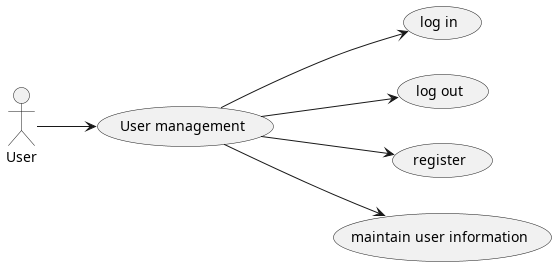
\includegraphics[width=0.94\linewidth]{userUserManagement}
    }
    \caption{Standard user}
  \end{subfigure}
  \hfill
  \noindent
  \begin{subfigure}{0.45\linewidth}
    \centering
    \fbox{
      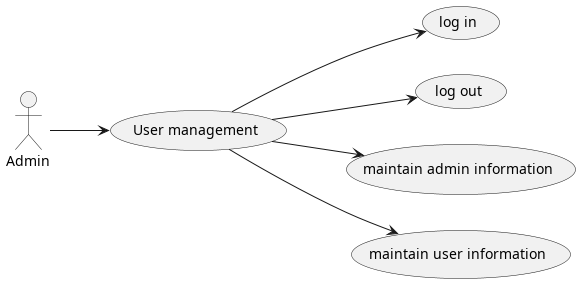
\includegraphics[width=0.92\linewidth]{adminUserManagement}
      }
    \caption{Administrator}
  \end{subfigure}
  \caption{User management}
\end{figure}
\usecasedesc
{Logging in}
{
  Users can signin / signup to the application by providing their username, email, password, and optionally their name, address, social network accounts, gender, birthday and a picture.

}
{
  This starts when a user wishes to log into the application.

  \paragraph{Basic Flows}
  \begin{itemize}
    \item Signin : if the user selected "Sign in” the Sign in sub flow is executed. The system requests that the user enter the login information (email \& password). Then :
    \begin{enumerate}
      \item If the user provides the requested information, the system validates the entered information and logs the user into the system.
      \item If the user selects "forgot password”  the system will ask the secret question and if the system validates, the user is logged in and he can modify his password else, he is redirected to the login page.
      \item If the user selects "Register”, the user will be redirect to the Register flow.
    \end{enumerate}
  \end{itemize}

  \paragraph{Alternative Flows}
  \begin{itemize}
    \item Invalid email/password : if in the Have an account flow, the user enters an invalid email and/or password, the system displays an error message. The user can choose to either return to the beginning of the Have an account flow or cancel the login, at which point the use case ends.
    \item Login canceled : if in the sign in sub flow the user decides not to login, the signin is canceled and the user is redirected to the log in sub flow.
  \end{itemize}
}
{None}
{None}
{If the log in was successful, the user is now logged into the system.  If not, the system state is unchanged.}
{None}

\usecasedesc
{Logging out}
{Users can also log out of the application}
{
  This starts when a user wishes to log out the application : the system logs out the user from the system.
}
{User must be logged in to log out}
{
  If the log out was successful, the user is now disconnected from the system and he will be redirected to the login page.
}
{None}
{None}

\usecasedesc
{Register}
{When a new user wants to use the application}
{
  The system requests that the user enter the register information. This includes :
  \begin{itemize}
    \item Name
    \item Birthdate
    \item Phone
    \item Email
    \item Password
    \item Secret question
    \item Allergies
  \end{itemize}

  \paragraph{Basic Flows}
  Once the user has provided the requested information, the system validates the entered information, generates and assigns a unique user id to the user. The user is added to the system and logs into the system.
  \paragraph{Alternative Flows}
  \begin{itemize}
    \item Invalid form : if the user enters an email already used or if another field of the form is wrong, the system displays an error message ("Something went wrong” for instance).
    \item Registration canceled : if in the Register sub flow the user decides not to register, the register is canceled and the user is redirected to the login sub flow.
  \end{itemize}
}
{None}
{User should not already have an account.}
{If the register was successful, the user is redirected to the home page.}
{None}

\usecasedesc
{Change information}
{
  This use case allows the user to maintain his personal information. This includes changing user information from the system. He can also ask for deleting his account.
}
{
  This use case begins when a user wants to change his information.

  The system requests that the user specify the function he/she would like to perform (either modify personal information or ask for deleting). Once the user has provided the requested information, one of the sub flows is executed

  \paragraph{Basic Flows}
  \begin{itemize}
    \item Change personal information : if the user selected "modify personal information", the modify personal information sub flow is executed :
    \begin{enumerate}
      \item The system retrieves his personal information and displays the user information. The user makes the desired changes to his information. This includes any of the information specified in the Register sub flow.
      \item Once the user has updated the necessary information, the system updates the user record with the updated information.
    \end{enumerate}
    \item Account deletion : If the user selected "Ask for deleting", the Ask for deleting sub flow is executed :
    \begin{enumerate}
      \item The system sends a notification to the administrator informing him that the user "X” wants to delete his account.
      \item The administrator can decide if he delete it or not. But as a GDPR compliant application, the administrator must delete the account if the user asks for it.
    \end{enumerate}
  \end{itemize}

  \paragraph{Alternative Flows}
  \begin{itemize}
    \item Modify personal information canceled : if in the modify personal information sub flow and the user decides not to modify his information, the modification is canceled and the user is redirected to the user page.
    \item Ask for deleting canceled : if in the ask for deleting sub flow and the user decides not to delete his account, the demand is canceled he is redirected to the user page.
  \end{itemize}
}
{None}
{User must be loggged in}
{If the use case was successful, the user information is updated from the system.  Otherwise, the system state is unchanged.}
{None}

\usecasedesc
{Administrator}
{
  This use case allows the administrator to maintain his personal information and maintain users. This includes changing his personal information from the system. He can also view the list of users and delete user account.
}
{
  The system requests that the administrator specify the function he/she would like to perform (either modify personal information or deleting).

  \paragraph{Basic Flows}
  \begin{itemize}
    \item If the administrator selected "modify personal information", the modify personal information subflow is executed :
    \begin{enumerate}
      \item The system retrieves his personal information and displays the administrator information.
      \item The administrator makes the desired changes to his information. This includes any of the information specified in the Register sub flow.
      \item Once the administrator has updated the necessary information, the system updates the user record with the updated information.
    \end{enumerate}
    \item If the administrator selected "view all users", the view user sub flow is executed :
    \begin{enumerate}
      \item The system retrieves the list of all users and displays it. The administrator has the list of all users.
      \item He can click and see all the information of a user.
    \end{enumerate}
    \item If the administrator selected "Delete a user ", the Delete a user sub flow is executed :
    \begin{enumerate}
      \item The administrator receive a notification that a user wants to delete his account.
      \item He decide to delete the account permanently or not (GDPR).
      \item If he decides to delete the account, an email will be sent to the user and the system updates the user record.
    \end{enumerate}

    \paragraph{Alternative Flows}
    \begin{itemize}
      \item Modify personal information canceled : if in the modify personal information sub flow the administrator decides not to modify his information, the modification is canceled and the administrator is redirected to the user page.
    \end{itemize}
  \end{itemize}

}
{None}
{The administrator must be logged in.}
{
  If the use case was successful, the administrator information is updated from the system and the user information is updated or deleted from the system. Otherwise, the system state is unchanged.
}
{None}